\documentclass[10pt]{article}
\usepackage[margin=1in]{geometry}
\usepackage{lmodern}
\usepackage[T1]{fontenc}
\usepackage{amsmath,amssymb,amsthm,booktabs,graphicx,microtype,enumitem,xcolor}
\usepackage[colorlinks=true,linkcolor=blue!50!black,urlcolor=blue!50!black]{hyperref}
\graphicspath{{figs/}}

\newtheorem{definition}{Definition}[section]
\newtheorem{proposition}{Proposition}
\newtheorem{theorem}{Theorem}
\newtheorem{lemma}{Lemma}
\theoremstyle{remark}
\newtheorem{remark}{Remark}
\newtheorem{finding}{Finding}
\newtheorem{question}{Q}

\newcommand{\HB}{\mathrm{HB}}
\newcommand{\Int}{\mathrm{Int}}
\newcommand{\Infer}{\mathrm{Infer}}
\newcommand{\val}{\mathrm{val}}
\newcommand{\lfp}{\mathrm{lfp}}
\newcommand{\Eval}{\mathrm{Eval}}
\newcommand{\eps}{\varepsilon}
\newcommand{\sut}{S}
\newcommand{\statusgood}[1]{\textbf{#1}}

\title{Accuracy Hides Semantic Error:\\
NeSyArena, a Measurement Instrument for Neuro-Symbolic Reasoning\\
\large Technical report and project record, v2 --- 2026-06-11}
\author{Ionel Eduard Stan \quad (with Claude as implementation collaborator)}
\date{}

\begin{document}
\maketitle

\begin{abstract}
\noindent
Neuro-symbolic (NeSy) reasoning systems are compared by task accuracy, yet accuracy cannot tell
whether a system computes the semantics it claims. We define \emph{semantic fidelity} --- the
signed, oracle-grounded error between the value a system computes and the value its declared
semantics defines --- and build \textsc{NeSyArena}, an open diagnostic instrument that measures it
under controlled program structure (proof multiplicity, overlap, recursion depth, aggregation
surrogates) together with its learning consequences (gradient liveness, calibration against exact
Bayes posteriors, held-out transfer). From an algebraic analysis of rule-based NeSy reasoning we
derive signed error laws for the common approximations and verify them to machine precision; the
laws are \emph{registered predictions}, and the instrument has by now \emph{refuted two of our own
registered hypotheses} --- the strongest evidence that it measures something derivation alone does
not give. Pointing the instrument at a deployed system produced a finding within a day: Scallop's
\texttt{addmultprob} under recursion computes proof-sums truncated at the tuple-set fixpoint
(neither distribution semantics nor infinitary proof-summing). End-to-end, task
accuracy is statistically indistinguishable across five reasoners while calibration and transfer
separate them decisively, on synthetic pixels and on real MNIST digits; a CLUTRR-style study shows
the truncation horizon reappearing as a systematic-generalization cliff at exactly the predicted
length. All generators, oracles, adapters, configurations and seeds are released; every number in
this report regenerates with one command.
\end{abstract}

\tableofcontents

%=====================================================================
\section{Reader's guide, project history, and why we pivoted}\label{sec:history}

This document is written for colleagues who need to understand --- and challenge --- what this
project claims. It is deliberately more complete than a conference paper: every symbol is defined
(\S\ref{sec:setting}, Appendix~\ref{app:notation}), every law is stated with proof
(\S\ref{sec:laws}), the methodology that protects the results is described
(\S\ref{sec:instrument}), the limitations are listed without euphemism (\S\ref{sec:limitations}),
and anticipated objections are answered explicitly (\S\ref{sec:faq}).

\subsection{Where the project comes from}

The project began as a theory paper submitted to KR~2026 (paper~305, \emph{A Semantics-First
Contract for Neuro-Symbolic Reasoning}). That paper factored rule-based NeSy systems into four
degrees of freedom --- a truth-value algebra $(V,\oplus,\otimes,0,1)$, body composition, derivation
aggregation, and a learnable base interpretation $f_\theta$ --- and proved two correspondence
theorems (restated as Theorems~\ref{thm:bounded} and \ref{thm:unbounded} below): bounded unrolling
needs only finitary semiring algebra, while unbounded recursion needs completeness and
$\omega$-continuity. An ``assumption stack'' turned this into a checklist for auditing systems.

The submission received three weak rejects. The criticisms, on re-reading, were substantially
correct, and the project's current shape is a direct response to them:

\begin{itemize}[leftmargin=2em]
\item \emph{``The math is semiring-PLP re-presented''} (Reviewer~C). Correct: the theorems are
semiring-valued versions of classical results (van Emden--Kowalski unfolding; Kleene fixed point),
already implicit in the provenance-semiring and algebraic-model-counting literature. Consequence:
the theorems are now \emph{cited background}, never the contribution.
\item \emph{``It only explains problems that were already found and fixed''} (Reviewer~B).
Correct as submitted: a checklist that post-dicts known bugs is not a result. Consequence: the
contribution must be an \emph{instrument} whose measurements produce new facts --- including facts
that contradict its authors' expectations. This report documents two such refutations
(\S\ref{sec:ledger}).
\item \emph{``Almost entirely theoretical''} (Reviewer~A). Correct. Consequence: the empirical
program of \S\S\ref{sec:conformance}--\ref{sec:learning}.
\end{itemize}

\subsection{The pivot, in one paragraph}

The pivot is from \emph{semantics as theory} to \emph{semantics as measurement}. The algebra stops
being the claim and becomes the calibration standard: for every system under test we fix the
semantics it \emph{claims} to compute, compute that semantics \emph{exactly} with an independent
oracle on the identical inputs, and report the signed difference as a function of program
structure. The theory's role is to generate falsifiable, signed, structural predictions (the error
laws of \S\ref{sec:laws}); the instrument's role is to confirm, refute, or refine them --- and to
measure what the theory underdetermines, which turned out to be where the interesting results are.

\subsection{Positioning in one sentence}

DeepLog, Scallop and Lobster are \emph{substrates} --- they execute a chosen semantics, by
compilation or by selectable provenance; \textsc{NeSyArena} is \emph{metrology} --- it measures
whether what a deployed system computes matches what it claims, and what the residual error does to
learning. The relationship is that of conformance test suites to compilers; \S\ref{sec:related}
develops this and \S\ref{sec:conformance} shows both kinds of substrate measured by the instrument.

%=====================================================================
\section{Formal setting}\label{sec:setting}

Everything in this section is standard or comes from the KR submission; it is the language the
instrument is built in. Appendix~\ref{app:notation} tabulates all notation.

\subsection{Programs}

\begin{definition}[Signature, atoms, Herbrand base]
A \emph{signature} $\Sigma$ consists of finitely many constants and predicate symbols. A
\emph{(ground) atom} is $p(c_1,\dots,c_k)$ with $p$ a $k$-ary predicate and $c_i$ constants. The
\emph{Herbrand base} $\HB(\Sigma)$ is the set of all ground atoms over $\Sigma$.
\end{definition}

\begin{definition}[Ground program; EDB/IDB]\label{def:program}
A \emph{ground rule} is $h \leftarrow b_1 \wedge \dots \wedge b_m$ with $h, b_i \in \HB(\Sigma)$.
A \emph{ground program} $\mathcal{P}$ is a finite set of ground rules. A predicate is
\emph{intensional} (IDB) if it occurs in some rule head, else \emph{extensional} (EDB). We write
$q$ for a distinguished \emph{query atom}.
\end{definition}

We work with ground programs throughout (the implementation grounds non-ground families during
generation); the positive (negation-free) fragment is the scope --- see \S\ref{sec:limitations}.

\subsection{Algebras}

\begin{definition}[Commutative semiring]\label{def:semiring}
$(V,\oplus,\otimes,0,1)$ where $(V,\oplus,0)$ and $(V,\otimes,1)$ are commutative monoids,
$\otimes$ distributes over $\oplus$, and $0$ is absorbing for $\otimes$. We read $\otimes$ as
composition along a rule body and $\oplus$ as aggregation over alternative derivations. $\oplus$ is
\emph{idempotent} if $a \oplus a = a$; idempotent $\oplus$ induces an order $a \le b
\Leftrightarrow a \oplus b = b$, making $\oplus$ a join.
\end{definition}

Instances used in this report: \textsc{Boolean} $(\{0,1\},\vee,\wedge)$ (we implement it as
$(\max,\min)$ on $[0,1]$, i.e.\ G\"odel), \textsc{maxprod} $([0,1],\max,\cdot)$,
\textsc{sumprod} $(\mathbb{R}_{\ge0},+,\cdot)$, \textsc{tropical}
$(\mathbb{R}_{\ge0}\cup\{\infty\},\min,+)$.

\begin{definition}[Quantale; $\omega$-continuity]\label{def:quantale}
A commutative \emph{quantale} is $(V,\le,\otimes,1)$ where $(V,\le)$ is a complete
join-semilattice (every subset has a supremum $\bigvee$) and $\otimes$ distributes over arbitrary
joins. An endofunction $F$ on a poset is \emph{$\omega$-continuous} if
$F(\bigvee_n x_n) = \bigvee_n F(x_n)$ for every increasing $\omega$-chain $(x_n)$.
\end{definition}

\subsection{Interpretations, the operator view, the proof view}

\begin{definition}[Interpretations; base interpretation]\label{def:base}
A \emph{$V$-interpretation} is $I : \HB(\Sigma) \to V$, ordered pointwise when $V$ is. The
\emph{base interpretation} $f_\theta : \HB(\Sigma) \to V$ supplies values for EDB atoms (in NeSy:
classifier outputs used as facts, with parameters $\theta$); by convention $f_\theta(a) = 0$ for
IDB atoms $a$, so derived atoms get their value from inference alone.
\end{definition}

\begin{definition}[Immediate consequence; bounded iteration]\label{def:tp}
For an interpretation $I$, body evaluation is $\Eval_I(b_1\wedge\dots\wedge b_m) = I(b_1) \otimes
\dots \otimes I(b_m)$, and
\[
(T_{\mathcal P} I)(a) \;=\; \bigoplus_{(a \leftarrow \beta)\in\mathcal P} \Eval_I(\beta),
\qquad
F^{f_\theta}_{\mathcal P}(I) \;=\; f_\theta \oplus T_{\mathcal P}(I)
\quad\text{(pointwise)},
\]
with $\bigoplus \emptyset = 0$. \emph{Bounded iteration}: $I^{(0)} = f_\theta$,\;
$I^{(n+1)} = F^{f_\theta}_{\mathcal P}(I^{(n)})$.
\end{definition}

\begin{definition}[Proof trees; depth; value]\label{def:proofs}
A \emph{proof tree} $\pi$ for $q$ is a finite tree with root labeled $q$; each internal node
labeled $a$ has children $b_1,\dots,b_m$ for some rule $a \leftarrow b_1\wedge\dots\wedge b_m \in
\mathcal P$; leaves are EDB atoms (or unexpanded atoms, which carry value $0$ and can be ignored).
$\mathrm{depth}(\pi)$ is the maximum root-to-leaf distance ($0$ for a single node). The
\emph{value} is $\val_{f_\theta}(\pi) = \bigotimes_{\ell \in \mathrm{leaves}(\pi)}
f_\theta(\ell)$, with leaf multiplicity (a fact used by two subtrees contributes twice under
non-idempotent $\otimes$). The \emph{support} $\mathrm{supp}(\pi)$ is the \emph{set} of its EDB
leaves. \emph{Depth-bounded proof aggregation}:
$\Infer^{(n)}(q) = \bigoplus_{\pi \,:\, \mathrm{depth}(\pi) \le n} \val_{f_\theta}(\pi)$.
\end{definition}

\subsection{The two correspondence theorems (cited background)}

\begin{theorem}[Bounded correspondence; KR submission Thm.~1]\label{thm:bounded}
Assume (i) finitely many ground rule instances per head atom, and (ii) $(V,\oplus,\otimes,0,1)$ a
commutative semiring. Then for every $n \in \mathbb N$ and ground $q$:\;
$I^{(n)}(q) = \Infer^{(n)}(q)$. Only \emph{finitary} algebra is needed.
\end{theorem}

\begin{theorem}[Unbounded correspondence; KR submission Thm.~2]\label{thm:unbounded}
Assume additionally that $(V,\le,\otimes,1)$ is a commutative quantale with $\oplus = \vee$ and
that $F^{f_\theta}_{\mathcal P}$ is $\omega$-continuous (which holds under countably many rule
instances per head). Then $I^\star := \lfp(F^{f_\theta}_{\mathcal P})$ exists by the Kleene
fixed-point theorem and $I^\star(q) = \bigvee_n \Infer^{(n)}(q)$ for every $q$.
\end{theorem}

\begin{remark}[Attribution and status]\label{rem:attribution}
These are semiring-valued forms of classical results (van Emden--Kowalski 1976; Lloyd 1987; Kleene)
in the lineage of provenance semirings (Green et al.\ 2007), algebraic model counting (Kimmig et
al.\ 2017), semiring Datalog convergence (Khamis et al.\ 2024) and Bourgaux et al.\ (2022). We do
not claim them; we \emph{verify them numerically inside the instrument}: operator iterates equal
proof aggregation, with proofs \emph{enumerated mechanically from the program IR}, to $10^{-12}$
on a cyclic program under non-idempotent $\oplus$ (\S\ref{sec:instrument}). The gap between
Theorem~\ref{thm:bounded} (cheap) and Theorem~\ref{thm:unbounded} (expensive assumptions) is
exactly where deployed systems improvise --- and where Finding~\ref{find:scallop} lives.
\end{remark}

\begin{definition}[Distribution semantics; WMC]\label{def:wmc}
Let the EDB atoms $f_1,\dots,f_m$ be independent Bernoulli facts with $\Pr(f_i) = p_i \in [0,1]$.
A \emph{world} $w \in \{0,1\}^m$ has probability $\pi(w) = \prod_i p_i^{w_i}(1-p_i)^{1-w_i}$. For
a monotone query $q$ whose proofs have supports $\sigma_1,\dots,\sigma_P \subseteq
\{f_1,\dots,f_m\}$, the \emph{distribution-semantics value} is the weighted model count
\[
P^*(q) \;=\; \Pr\Bigl(\,\bigcup_{j} E_{\sigma_j}\Bigr)
\;=\; \sum_{w \,:\, w \models q} \pi(w),
\qquad E_\sigma = \textstyle\bigwedge_{f\in\sigma} f .
\]
Computing $P^*$ correctly requires a disjoint representation (knowledge compilation / AMC), not
proof enumeration: proof-sums double count.
\end{definition}

%=====================================================================
\section{Semantic fidelity: the measurement framework}\label{sec:framework}

\subsection{Claimed semantics and the central definition}

\begin{definition}[Claimed semantics; oracle]\label{def:claimed}
A \emph{system under test} (SUT) $\sut$ declares a \emph{claimed semantics}: the mathematical
object it purports to compute (e.g.\ ``distribution semantics'', ``max-join over proof scores'',
``least fixed point under $(\max,\cdot)$''). The \emph{oracle value} $I^*(q)$ is that object
computed exactly, by an independent method, from the \emph{identical} base interpretation
$f_\theta$ the SUT consumes.
\end{definition}

\begin{definition}[D1: semantic error]\label{def:error}
$\eps_\sut(q) \;=\; \hat\sut(q) - I^*(q)$, where $\hat\sut(q)$ is what the SUT returns. Signed by
design: over- and under-counting are different failure modes with different learning consequences.
Because oracle and SUT share $f_\theta$, $\eps$ isolates the \emph{reasoning} layer from
perception.
\end{definition}

\begin{definition}[D2: fidelity profile]\label{def:profile}
For structured sweep families $\{G_a\}$, one per diagnostic axis $a$ (\S\ref{sec:generators}),
$\phi_a(\sut) = \max\bigl(0,\, 1 - \mathbb{E}_{G_a}\lvert\eps_\sut\rvert\bigr)$. The vector
$\phi(\sut)$ is the scorecard (Figure~\ref{fig:radar}); raw signed errors are always reported
alongside.
\end{definition}

\begin{definition}[D3: depth horizon]\label{def:horizon}
On a family with required proof depth $L$ (chains), $h_\delta(\sut) = \min\{L :
\lvert\eps_\sut\rvert > \delta\}$. For an $n$-step unroller, Theorem~\ref{thm:bounded} predicts
$h_\delta = n+1$.
\end{definition}

\begin{definition}[D4: gradient liveness]\label{def:liveness}
With oracle gradient $\nabla^*$ and system gradient $\hat\nabla$ (each system differentiates
\emph{its own} value function --- see Def.~\ref{def:suts}),
\[
\mathrm{live}(\sut) = \frac{\#\{f : \lvert\hat\nabla_f\rvert > \tau \wedge
\lvert\nabla^*_f\rvert > \tau\}}{\#\{f : \lvert\nabla^*_f\rvert > \tau\}},
\]
the share of facts the oracle would update that the SUT also updates ($\tau = 10^{-12}$ for
analytic gradients, $10^{-9}$ in batched settings).
\end{definition}

\begin{definition}[D5: learning-consequence metrics]\label{def:learning-metrics}
In learning experiments the perception module is trained \emph{through} each SUT and evaluated
against exact ground truth: \emph{calibration} = mean $\lvert p_{\text{percept}} -
p_{\text{Bayes}}\rvert$ where the Bayes posterior is closed-form by construction of the generative
model; \emph{transfer} = mean $\lvert \hat\sut(q_h; \text{learned } f_\theta) - I^*(q_h;
\text{true } f_\theta)\rvert$ over held-out queries $q_h$, i.e.\ deployment error of the whole
trained pipeline; \emph{facts-quality} = the same with the \emph{exact} reasoner substituted at
deployment, isolating perception corruption from deployment-time reasoning error. The
\emph{oracle floor} is the exact-trained pipeline's value: irreducible estimation error.
\end{definition}

\begin{definition}[D6: witness]\label{def:witness}
A minimal generator configuration $g$ with $\lvert\eps_\sut(g)\rvert > \delta$, found by ordered
grid search followed by greedy shrinking along each parameter (QuickCheck-style). Witnesses are
the machine-found analogue of hand-crafted failure micro-examples.
\end{definition}

\subsection{The reference systems under test}

\begin{definition}[Reference SUTs and their gradient semantics]\label{def:suts}
Let $q$ have proof supports $\sigma_1,\dots,\sigma_P$ and scores $s_j = \prod_{f\in\sigma_j} p_f$.
The five reference SUTs, each mirroring a deployed aggregation strategy \emph{including its
differentiation behavior}:
\begin{itemize}[leftmargin=2em]
\item \textbf{exact-wmc}: $P^*(q)$ (Def.~\ref{def:wmc}); gradient analytic
  (Prop.~\ref{prop:grad}). Claimed semantics: distribution semantics; $\eps \equiv 0$ by
  definition.
\item \textbf{add-mult(clamped)}: $\min(1, \sum_j s_j)$. Gradient: $\partial/\partial p_f \sum_j
  s_j$ when the sum is $<1$; \emph{identically zero} when $\ge 1$ (the clamp's flat region ---
  ``gradient blackout''). Claim: distribution semantics.
\item \textbf{top-$k$}: $P^*$ restricted to the $k$ highest-scoring proofs; the selection is
  \emph{frozen} (not differentiated through), gradients flow through the restricted WMC
  (difftopkproofs-style). Claim: distribution semantics.
\item \textbf{min-max}: $\max_j \min_{f\in\sigma_j} p_f$; subgradient is \emph{one-hot} at the
  bottleneck fact of the best proof (ties broken lexicographically --- a deliberate, documented
  determinism fix over the toy, whose tie depended on hash order). Claim: distribution semantics.
\item \textbf{LSE$_\tau$}: $\tau\log\sum_j e^{s_j/\tau}$, the smooth surrogate for the max-join;
  its \emph{claimed} semantics is $\max_j s_j$ (so its oracle is the max, not WMC); softmax-weighted
  gradients.
\end{itemize}
\end{definition}

\begin{remark}[Why reference SUTs and not only deployed systems]\label{rem:why-refs}
The reference SUTs are exactly specified, fast, and differentiable with controlled semantics; the
deployed systems are then \emph{measured against them} (\S\ref{sec:conformance}). The measured
result --- agreement at machine precision on the acyclic battery --- is what authorizes
transferring every reference-SUT result to the deployed systems. Where deployed behavior
\emph{deviates} from the reference model (recursion; Finding~\ref{find:scallop}), the deviation
itself is the result.
\end{remark}

%=====================================================================
\section{Error laws}\label{sec:laws}

Each law converts one violated algebraic commitment into a \emph{signed, registered prediction}.
They are deliberately elementary; their value is falsifiability, not depth. All were verified to
the stated precision by the rebuilt instrument.

\begin{proposition}[Proof-sums over-count; clamp blacks out]\label{prop:addmult}
With events $E_j = E_{\sigma_j}$ (Def.~\ref{def:wmc}),
\[
0 \;\le\; \sum_{j} s_j - P^*(q) \;\le\; \sum_{i<j} \Pr(E_i \wedge E_j),
\]
with equality on the left iff the $E_j$ are pairwise disjoint. Moreover
$\min(1,\sum_j s_j)$ has identically zero gradient wherever $\sum_j s_j \ge 1$.
\end{proposition}
\begin{proof}
$s_j = \Pr(E_j)$ under independent facts. The union bound gives $P^* = \Pr(\bigcup E_j) \le \sum_j
\Pr(E_j)$, i.e.\ the left inequality; Bonferroni's second-order lower bound gives $\Pr(\bigcup
E_j) \ge \sum_j \Pr(E_j) - \sum_{i<j}\Pr(E_i\wedge E_j)$, i.e.\ the right. Equality on the left
iff no overlap mass, i.e.\ pairwise disjointness. The clamp claim is immediate: $x \mapsto
\min(1,x)$ is constant on $[1,\infty)$. \emph{Status: verified; the Bonferroni upper bound is
asserted in the standing test battery; witness $+0.160$ at $(P,L,c,p)=(2,1,0,0.6)$.}
\end{proof}

\begin{proposition}[Top-$k$ under-counts by at most the dropped mass]\label{prop:topk}
Let $K$ be the set of $k$ highest-scoring proofs. Then
\[
0 \;\le\; P^*(q) - \Pr\Bigl(\bigcup_{j \in K} E_j\Bigr) \;\le\; \sum_{j \notin K} s_j ,
\]
zero iff every dropped proof is covered (almost surely) by the kept union; in particular
$\eps = 0$ whenever $P \le k$.
\end{proposition}
\begin{proof}
Monotonicity of probability gives the left inequality. For the right:
$\Pr(\bigcup_{\text{all}}) - \Pr(\bigcup_K) \le \Pr(\bigcup_{j\notin K} E_j) \le \sum_{j\notin K}
\Pr(E_j)$. \emph{Status: verified; witnesses $-0.210$ ($k{=}1$) and $-0.103$ ($k{=}3$); the
$k \ge P$ identity is additionally measured end-to-end in both learning controls
(\S\ref{sec:learning}).}
\end{proof}

\begin{proposition}[Surrogate bias law]\label{prop:lse}
For scores $s_1,\dots,s_P$, $P \ge 2$:
$\max_j s_j \;<\; \mathrm{LSE}_\tau(s_1,\dots,s_P) \;\le\; \max_j s_j + \tau\ln P$,
with equality on the right iff all scores are equal; for equal scores the bias is exactly
$\tau\ln P$.
\end{proposition}
\begin{proof}
Write $M = \max_j s_j$. Strict lower bound: $\sum_j e^{s_j/\tau} > e^{M/\tau}$ since the other
$P-1$ terms are positive. Upper bound: $\sum_j e^{s_j/\tau} \le P\,e^{M/\tau}$, so
$\mathrm{LSE}_\tau \le M + \tau\ln P$, with equality iff every $s_j = M$. \emph{Status: verified to
$2.22\times10^{-16}$ over a $(P,\tau)$ grid.}
\end{proof}

\begin{proposition}[Truncation starves gradients]\label{prop:trunc}
If the minimal proof depth of $q$ exceeds the unrolling budget $n$ (and $f_\theta$ assigns $0$ to
IDB atoms), then $I^{(n)}(q) = 0$ and $\nabla_\theta\, I^{(n)}(q) \equiv 0$.
\end{proposition}
\begin{proof}
By Theorem~\ref{thm:bounded}, $I^{(n)}(q) = \Infer^{(n)}(q)$, and the depth-$\le n$ proof set is
empty, so $I^{(n)}(q) = \bigoplus\emptyset = 0$ \emph{identically in a neighborhood of} $\theta$:
perturbing fact values creates no proof of depth $\le n$. A constant function has zero gradient.
\emph{Status: verified --- value and finite-difference gradient exactly $0$ below the horizon;
measured horizons equal $n+1$ for $n \in \{2,4,6,8,10\}$; end-to-end consequences in E7 and E8.}
\end{proof}

\begin{proposition}[Analytic WMC gradient]\label{prop:grad}
For $P^*(q)$ as in Def.~\ref{def:wmc} and any fact $f$ with $p_f \in (0,1)$:
\[
\frac{\partial P^*(q)}{\partial p_f} \;=\; \Pr(q \mid f) - \Pr(q \mid \neg f)
\;=\; \sum_{w \,:\, w\models q} \pi(w)\,\frac{w_f - p_f}{p_f\,(1-p_f)} .
\]
\end{proposition}
\begin{proof}
Split the worlds by $w_f$: $P^* = p_f \Pr(q\mid f) + (1-p_f)\Pr(q\mid\neg f)$, where the
conditional terms do not depend on $p_f$; differentiate. The second form follows since
$\pi(w)/p_f$ (resp.\ $\pi(w)/(1-p_f)$) is the conditional world probability. \emph{Status: matches
finite differences to $10^{-6}$ (step $10^{-7}$) and is the oracle for all gradient-conformance
comparisons.}
\end{proof}

\begin{remark}[What the laws do \emph{not} determine]
The laws bound each error in isolation. They do not determine (i) the crossover point where the
$\lvert\eps\rvert$-ranking of over- and under-counting flips (measured: between $c{=}1$ and
$c{=}2$ at $P{=}4, L{=}4, p{=}0.6$); (ii) the sign of min-max error (measured: structure-dependent,
$+0.39$ vs $-0.47$ in the toy study); (iii) any of the learning-time interactions of
\S\ref{sec:learning}. That gap is the argument for the instrument.
\end{remark}

%=====================================================================
\section{The instrument and its methodology}\label{sec:instrument}

\subsection{Architecture}

The rebuilt codebase (\texttt{src/nesyarena/}, 107 tests) is organized as:
\begin{center}\small
\begin{tabular}{ll}
\toprule
\texttt{ir.py} & ground-program IR: \texttt{Atom}/\texttt{Rule}/\texttt{GroundProgram};
bounded proof enumeration\\
\texttt{algebra.py} & semiring registry (\textsc{boolean}, \textsc{maxprod}, \textsc{sumprod},
\textsc{tropical})\\
\texttt{engine.py} & $T_{\mathcal P}$ iteration, run-to-convergence, proof-side aggregation\\
\texttt{oracle.py} & brute-force WMC ($m \le 22$) + analytic gradients; ProbLog oracle; graph
oracles\\
\texttt{suts.py} & the five reference SUTs of Def.~\ref{def:suts}\\
\texttt{generators.py} & program families G1--G3 (\S\ref{sec:generators})\\
\texttt{metrics.py}, \texttt{witness.py} & D2--D4, D6\\
\texttt{learning/} & batched torch provenance layer whose \emph{plain autograd} is
system-faithful\\
\texttt{adapters/} & frozen adapter protocol; Scallop, DeepLog\\
\bottomrule
\end{tabular}
\end{center}
Programs are the primary object: generators emit programs, proof sets are \emph{derived} by
bounded enumeration (dual view: leaf multisets for semiring evaluation; support sets as the DNF
for WMC), and external adapters compile the same object. One documented caveat: enumeration
identifies proof trees by leaf multiset; two distinct trees with identical multisets would
collapse, which matters only under non-idempotent $\oplus$ and cannot occur on the families used
(one rule per proof; transitive closure, where derivations are walks with unique edge multisets).

\subsection{Generators (exact specifications)}\label{sec:generators}

\begin{itemize}[leftmargin=2em]
\item \textbf{G1 (overlap).} Parameters $(P, L, c, p)$, optionally heterogeneous: query $q$ with
$P$ proofs, each of length $L$, sharing $c$ ``trunk'' facts; private facts $x_{j,i}$; all
probabilities $p$, or i.i.d.\ $U[0.35, 0.9]$. Fact count $m = c + P(L-c) \le 22$. Axes:
multiplicity ($P$), overlap ($c$), saturation ($p$ high).
\item \textbf{G2 (depth).} Chains $v_0 \to \dots \to v_L$ with edge probability $p$, transitive
closure program, query $\mathrm{path}(v_0, v_L)$ (minimal proof depth $L$); the cyclic instance $a
\leftrightarrow b \to c$ ($p_{ab}=p_{ba}=0.9$, $p_{bc}=0.8$) as the canonical recursion stress
(infinitely many proofs).
\item \textbf{G3 (surrogate).} Score multisets as single-fact proofs: equal scores $(s, P)$ for
the bias law; one boosted proof ($s + \Delta$) for the dilemma curve.
\item \textbf{E8 generator (CLUTRR-style lineal kinship).} Relations $=$ (gender, generation
offset) with offset in $[-2,2]$ (10 relations; 6 base relations with $\lvert d\rvert\le1$);
composition $(g_1,d_1)\circ(g_2,d_2) = (g_2, d_1{+}d_2)$, deterministic and closed; chains sampled
with all prefix offsets in range.
\end{itemize}

\subsection{Oracles and the validation chain}\label{sec:validation}

The distribution-semantics oracle enumerates all $2^m$ worlds ($m \le 22$) and computes $P^*$ and
its analytic gradient (Prop.~\ref{prop:grad}) in one vectorized pass; beyond $m = 22$, ProbLog's
exact inference (knowledge compilation) is the oracle. Idempotent algebras on transitive closure
use direct graph algorithms. \emph{The oracle never rests on itself}: the standing test battery
asserts brute-force $\equiv$ ProbLog to $<10^{-10}$ on random instances (measured
$6.7\times10^{-16}$), analytic $\equiv$ finite-difference gradients, and
Theorem~\ref{thm:bounded} numerically on the cyclic program under \textsc{sumprod} for $n =
0..10$ with proofs enumerated from the IR.

\subsection{Methodological safeguards}\label{sec:method}

\begin{enumerate}[leftmargin=2em]
\item \textbf{Registered predictions.} Every error law and every hypothesis carries its predicted
sign and growth direction \emph{written before the run} (in configs and docstrings); outcomes are
recorded either way. The ledger (\S\ref{sec:ledger}) contains two refutations of our own
predictions --- the discipline is load-bearing, not decorative.
\item \textbf{Parity gates.} The first implementation (the ``toy'', now \texttt{legacy/}) was
verified, then frozen as an \emph{executable specification}: golden fixtures pin its oracle
values, gradients, engine trajectories and witnesses; the rebuilt core must reproduce them
(tolerances $10^{-10}$--$10^{-14}$). Learning experiments were re-implemented on torch autograd
and reproduce the toy's numpy results \emph{to every printed decimal including standard
deviations} --- two independent implementations following identical trajectories.
\item \textbf{Shared inputs.} Oracle and SUT always consume the identical $(\mathcal P,
f_\theta)$; in learning runs all SUTs share data, seeds, and initializations within a seed.
\item \textbf{No silent coverage loss.} Sweep cells skipped (e.g.\ over the WMC fact limit) are
logged in the output; configs are committed YAML whose sha256 is embedded in every result file.
\item \textbf{Adapters never normalize.} A deployed system's deviation from its claim must pass
through the adapter verbatim; deviations are findings, pinned by canary tests that flip if
upstream changes (versions pinned).
\item \textbf{One-command reproduction.} \texttt{make all} regenerates every number and figure in
this report (Appendix~\ref{app:repro}).
\end{enumerate}

%=====================================================================
\section{Conformance of deployed systems}\label{sec:conformance}

Two deployed backends were measured. Versions: scallopy 0.2.4 (official release wheel);
pydeeplog 3.0.3 (PyPI; repo ML-KULeuven/deeplog, last push 2026-06-03); ProbLog 2.2.10.

\subsection{Scallop: value and gradient conformance, then a recursion finding}

On 50 G1 instances (homogeneous and heterogeneous), Scallop's provenances match the reference
SUTs at machine precision while deviating from the exact oracle by the magnitudes the laws
predict:

\begin{center}\small
\begin{tabular}{lcc}
\toprule
provenance & $\max\lvert\text{scallop} - \text{reference}\rvert$ &
$\max\lvert\text{scallop} - \text{oracle}\rvert$\\
\midrule
addmultprob & $2.2\times10^{-16}$ & $0.609$\\
minmaxprob & $0.0$ & $0.263$\\
topkproofs($k{=}1$) & $5.6\times10^{-17}$ & $0.378$\\
topkproofs($k{=}3$) & $2.2\times10^{-16}$ & $0.061$\\
\bottomrule
\end{tabular}
\end{center}

\noindent The same conformance holds through full program compilation (the IR adapter), on chains
run by Scallop's native recursion (agreement $0.0$ with the convergent fixpoint), and at the
\emph{gradient} level: central finite differences through Scallop match the references'
system-faithful gradients to $7.9\times10^{-12}$ on tie-free instances --- confirming frozen
top-$k$ selection and the one-hot min-max subgradient as deployed differentiation behavior.
Deployed Scallop exposes no bounded-iteration mode through scallopy 0.2.4 (run-to-fixpoint only),
so the depth axis applies to it only via program rewriting.

\begin{finding}[Scallop's \texttt{addmultprob} under recursion is not proof-summing]
\label{find:scallop}
On the cyclic instance, the naive model of add-mult --- sum all (bounded-depth) proof scores,
clamp at 1 --- predicts $1.0$; deployed Scallop returns $0.72$. A designed probe isolates the
mechanism (diamond $a{\to}b{\to}c$, $a{\to}d{\to}c$ with $0.6$ edges, $\pm$ a back-edge
$c{\to}a$): on the DAG, Scallop returns exactly the simple-path proof-sum ($0.720$ vs oracle
$0.5904$ --- the predicted rung-P over-count); adding the cycle changes \emph{nothing}.
Derivations that re-derive an already-present tuple never accumulate into its tag: iteration stops
at the \emph{tuple-set} fixpoint, freezing tags at their acyclic-derivation values. The deployed
semantic object under recursion is therefore \emph{iteration-policy-dependent} --- neither
distribution semantics nor infinitary proof-summing. Two consequences: (i) on cyclic
reachability this accidentally \emph{protects} addmultprob from divergence/saturation (a
coincidence of subsumed loop supports, not a guarantee); (ii) the reference AddMult remains a
faithful model of deployed behavior on acyclic structure --- where the overlap axis lives --- but
recursive sweeps require a truncated-at-tuple-fixpoint reference variant (not yet implemented;
\S\ref{sec:limitations}).
\end{finding}

\subsection{DeepLog: conformance pass, including gradients}

DeepLog compiles formula specifications to algebraic circuits and claims exactness. Registered
prediction: fidelity $1.0$ at the circuit's working precision. Measured: the
weighted-model-count construction (assignment-aware $p(F)$ weights $\times$ boolean-to-probability
transform of the proof DNF) matches the WMC oracle to $<10^{-6}$ on the G1 battery (float32
circuits); recursion handled by the arena's bounded unrolling is exact. Gradients: symbolic
(non-numeric) probability labels survive DeepLog's label resolver and surface as module inputs, so
torch autograd through the compiled circuit yields DeepLog's \emph{deployed} gradients ---
matching the analytic oracle gradient to $1.3\times10^{-7}$. A conformance \emph{pass} is as much
a result as a deviation: it is what makes the leaderboard contrast (exact substrate vs approximate
provenances) a measurement rather than an assertion.

\begin{remark}[Why the finding matters beyond bug-hunting]
F-\ref{find:scallop} is an \emph{implicit semantics choice} (iteration policy under recursion),
invisible to accuracy-style evaluation and found within hours of pointing the instrument at the
system. This is the thesis demonstrating itself: claimed semantics must be measured, not assumed.
\end{remark}

%=====================================================================
\section{Inference-level results (E1--E4)}\label{sec:inference}

\paragraph{E1 --- structural crossover.}
On the G1 grid (1030 cells; skipped cells logged), add-mult's signed error grows with overlap
($+0.092 \to +0.308$ as $c: 0\to3$ at $P{=}4, L{=}4, p{=}0.6$) while top-1's shrinks ($-0.296 \to
-0.081$): opposite monotone structural sensitivities, with the $\lvert\eps\rvert$-ranking flipping
between $c{=}1$ and $c{=}2$ (Fig.~\ref{fig:crossover}). \emph{No method dominates; structure
decides.} Grid-level fidelity $\phi_{\text{overlap}}$: exact $1.0$; top-3 $0.970$; add-mult
$0.863$; top-1 $0.857$; min-max $0.823$.

\paragraph{E2 --- depth horizons and recursion stress.}
Measured horizons are exactly $n{+}1$ for $n \in \{2,4,6,8,10\}$ (none within range for $n \ge
12$, logged as such); below the horizon the value is flat zero (finite-difference liveness $0$ on
every $(n, L{=}n{+}1)$ cell); at the horizon, values match theory to $5\times10^{-7}$ ($0.430467 =
0.9^8$, $0.478297 = 0.9^7$). On the cyclic instance, run-to-convergence \textsc{sumprod} reaches
$3.7895 = 0.72/0.19 > 1$ --- the H7 ``probability'' leaving $[0,1]$ --- while \textsc{maxprod}
correctly converges to $0.72$ (Fig.~\ref{fig:horizon}).

\paragraph{E3 --- the surrogate dilemma.}
The bias law holds to $2.22\times10^{-16}$ across $(P,\tau)$; plotting bias against the gradient
share reaching non-maximal proofs shows the unreachable corner: no temperature achieves both low
bias and live gradients (Fig.~\ref{fig:surrogate}).

\paragraph{E4 --- witnesses.}
The synthesizer, given only ``find the smallest failing configuration'', returns:
add-mult $(P,L,c,p) = (2,1,0,0.6)$, $\eps = +0.160$ (re-deriving the canonical double-counting
micro-example from the literature); top-1 $(2,1,0,0.3)$, $-0.210$; top-3 $(4,1,0,0.3)$, $-0.103$;
min-max $(1,2,0,0.3)$, $+0.210$ --- notably min-max fails on a \emph{single} proof of two facts:
it does not need alternative derivations to be wrong. Exact-WMC has no witness on the grid.

\paragraph{Gradient liveness ladder (radar axis).}
exact $1.000$; top-3 $0.832$; add-mult $0.611$ (clamp blackout); top-1 $0.498$; min-max $0.166
\approx 1/m$ (the one-hot subgradient keeps a single fact alive).

\begin{figure}[t]\centering

\includegraphics[width=.58\linewidth]{F2_crossover.png}
\caption{E1: opposite structural sensitivities of over- and under-counting approximations
($P{=}4$, $L{=}4$, $p{=}0.6$); the ranking flips between $c{=}1$ and $c{=}2$.}
\label{fig:crossover}
\end{figure}

\begin{figure}[t]\centering

\includegraphics[width=.92\linewidth]{F3_depth_horizon.png}
\caption{E2: truncation values fall to flat zero past the horizon (left); measured horizons sit
exactly on the $n{+}1$ line (right).}
\label{fig:horizon}
\end{figure}

\begin{figure}[t]\centering
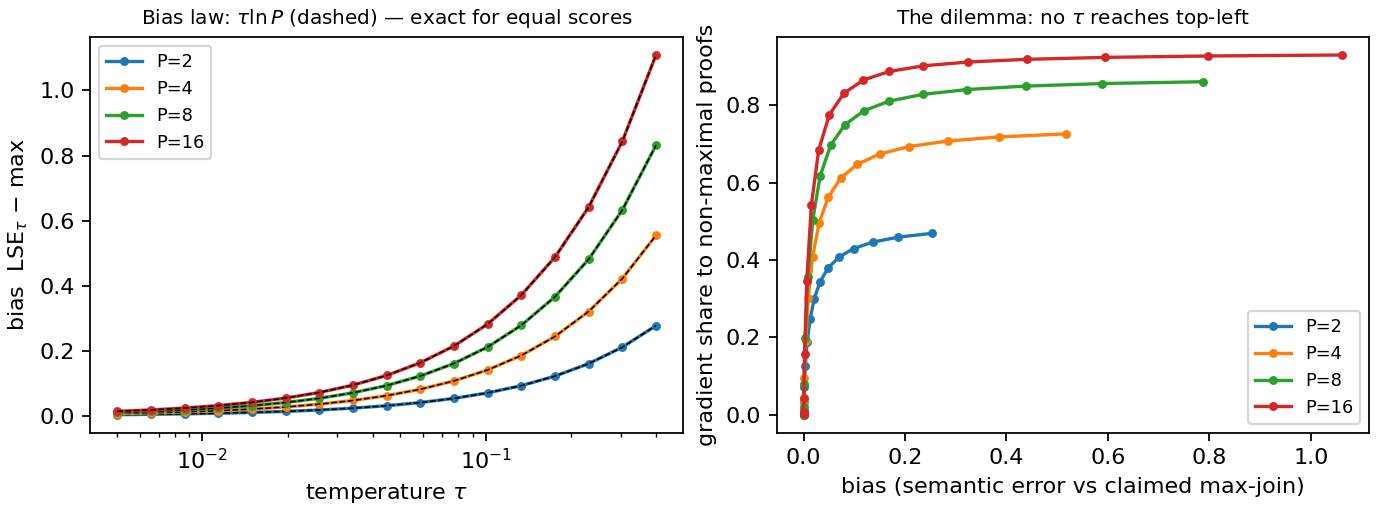
\includegraphics[width=.92\linewidth]{F4_surrogate.png}
\caption{E3: the $\tau\ln P$ bias law (left, dashed = closed form) and the temperature dilemma
(right): no $\tau$ reaches the low-bias/live-gradients corner.}
\label{fig:surrogate}
\end{figure}

\begin{figure}[t]\centering

\includegraphics[width=.5\linewidth]{scorecard_radar.png}
\caption{Measured fidelity profiles $\phi$ over six axes (multiplicity, overlap, saturation,
gradient liveness, fact-table transfer, pixel transfer efficiency).}
\label{fig:radar}
\end{figure}

%=====================================================================
\section{Learning-level results (E5--E8)}\label{sec:learning}

The learning layer implements each SUT as a batched torch operation whose \emph{plain autograd}
reproduces the system-faithful gradients of Def.~\ref{def:suts} (parity-gated to $10^{-10}$):
clamp via \texttt{torch.clamp}, frozen selection via detached argsort, one-hot subgradients via
\texttt{amin}/\texttt{amax}. Training code is therefore ordinary \texttt{loss.backward()}, and
each reasoner's distortions reach the perception module exactly as deployed systems deliver them.

\subsection{E6, fact-table setting (population-loss limit; 5 seeds)}

A free fact table $\theta \in \mathbb{R}^m$ (probabilities $\sigma(\theta)$) is trained through
each reasoner. \emph{Treatment}: G1$(4,3,2)$ with heterogeneous ground-truth probabilities;
supervision is a 7-query battery (the 6 proof-pairs and the full union) with exact-WMC targets;
evaluation is held-out queries (4 singletons + one triple) against exact ground truth, aggregated
by the \emph{same} reasoner at deployment. \emph{Control}: the categorical-sum structure
(MNIST-sum$_2$ shape, $\lvert\text{dom}\rvert = 3$): mutually exclusive proofs, where
Prop.~\ref{prop:addmult} predicts add-mult is \emph{exactly} distribution semantics; exact and
add-mult share one code path so the identity is structural.

\begin{center}\small
\begin{tabular}{lcccc}
\toprule
SUT & control (disjoint) & treatment (overlap) & facts-quality & fact MAE\\
\midrule
exact & $0.010 \pm 0.020$ & $0.000 \pm 0.000$ & $0.000$ & $0.029$\\
add-mult & $0.010 \pm 0.020$ & $0.101 \pm 0.029$ & $0.123$ & $0.128$\\
top-1 & $0.148 \pm 0.076$ & $0.109 \pm 0.052$ & $0.113$ & $0.191$\\
top-3 & $0.010 \pm 0.020$ & $0.004 \pm 0.003$ & $0.004$ & $0.041$\\
min-max & $0.071 \pm 0.059$ & $0.095 \pm 0.045$ & $0.212$ & $0.272$\\
\bottomrule
\end{tabular}
\end{center}

\noindent Reading: training through a misreasoner corrupts the \emph{learned facts themselves}
(fact MAE $0.13$--$0.27$ vs $0.03$), not just deployment values; on the disjoint control,
double-counting is invisible (exact $=$ add-mult) --- precisely the cell of the structure grid
where the field's default benchmark lives --- while truncation (top-1) is what such tasks
\emph{can} see. This is the benchmark autopsy (H9) as a learning experiment.

\subsection{E6, pixel perception (the H8 headline; 3 seeds)}

Perception is an MLP on synthetic $8{\times}8$ images whose generative model is known, so the
Bayes posterior is closed-form and calibration is measured against exact ground truth
(Def.~\ref{def:learning-metrics}). Trained end-to-end through each reasoner on sampled binary
labels (Fig.~\ref{fig:pixels}):

\begin{center}\small
\begin{tabular}{lcccc}
\toprule
SUT & accuracy & calibration vs Bayes & transfer & facts-quality\\
\midrule
exact & $0.740 \pm 0.004$ & $0.101 \pm 0.003$ & $0.062 \pm 0.002$ & $0.062 \pm 0.002$\\
add-mult & $0.734 \pm 0.006$ & $0.145 \pm 0.002$ & $0.093 \pm 0.002$ & $0.101 \pm 0.002$\\
top-1 & $0.744 \pm 0.005$ & $0.105 \pm 0.004$ & $0.068 \pm 0.003$ & $0.069 \pm 0.003$\\
top-3 & $0.740 \pm 0.004$ & $0.101 \pm 0.003$ & $0.063 \pm 0.003$ & $0.063 \pm 0.003$\\
min-max & $0.742 \pm 0.007$ & $0.128 \pm 0.002$ & $0.085 \pm 0.004$ & $0.084 \pm 0.001$\\
\bottomrule
\end{tabular}
\end{center}

\noindent \textbf{Accuracy is statistically indistinguishable across all five reasoners
($0.734$--$0.744$) while calibration and transfer separate them decisively}: add-mult sits $44\%$
above the calibration floor and $50\%$ above the transfer floor. On the sum-structured control,
exact $\equiv$ add-mult $\equiv$ top-3 to every decimal (top-3 measured through the top-$k$ code
path), while top-1 is harmed --- the autopsy again.

\emph{Setting dependence, resolved by a registered ablation (toy study).} Top-1, harmful in the
fact-table setting, matches the oracle floor under pixel parameterization. We registered the
hypothesis (H-A) that supervision richness explains this; the ablation \emph{refuted} it: top-1
ties the floor under both single-query and battery supervision; the operative variable is
\emph{parameterization} --- a shared perception network absorbs truncation bias that a free fact
table amplifies. Add-mult is harmed under both regimes, and decomposes: battery supervision
repairs its perception calibration ($0.175 \to 0.095$) but \emph{not} deployment transfer
($0.117$), because held-out queries are still aggregated by the faulty reasoner at inference time.
(Provenance note: H-A's numbers are from the verified toy study and are not yet re-run on the
rebuilt harness; see \S\ref{sec:limitations}.)

\subsection{E5, MNIST scale (real digits; 3 seeds)}

\emph{MNIST-path} (treatment): a $3{\times}3$ grid of MNIST digits; a cell is open iff its digit
is even; the query is monotone corner-to-corner reachability --- 6 paths of 5 cells, genuinely
overlapping. \emph{MNIST-sum} (control): digit pairs from $\{0,1,2\}$, train on the sum query
(mutually exclusive proofs), transfer to the equality query. Real images have no closed-form
Bayes posterior, so this experiment measures the accuracy-vs-transfer divergence (perception
quality against true cell states), not exact calibration.

\begin{center}\small
\begin{tabular}{lccc}
\toprule
\multicolumn{4}{c}{MNIST-path treatment}\\
SUT & accuracy & perception MAE & transfer\\
\midrule
exact & $0.952 \pm 0.003$ & $0.097 \pm 0.008$ & $0.031 \pm 0.001$\\
add-mult & $0.934 \pm 0.006$ & $0.160 \pm 0.016$ & $0.040 \pm 0.002$\\
top-1 & $0.951 \pm 0.002$ & $0.095 \pm 0.006$ & $0.031 \pm 0.001$\\
top-3 & $0.952 \pm 0.004$ & $0.097 \pm 0.009$ & $0.031 \pm 0.001$\\
min-max & $0.940 \pm 0.006$ & $0.140 \pm 0.006$ & $0.038 \pm 0.002$\\
\bottomrule
\end{tabular}
\end{center}

\noindent The synthetic findings replicate on real digits: add-mult corrupts perception ($+65\%$
MAE over the floor) and transfer ($+29\%$) while accuracy moves by at most $\sim$2 points. On the
control, exact $\equiv$ add-mult $\equiv$ top-3 again --- and a \emph{surprise}: top-1
\emph{beats} exact on transfer ($0.019$ vs $0.221$).

\subsection{E5b, the knife-edge ablation (registered; one prediction refuted)}

We hypothesized (H-N) that top-1's control win comes from near-deterministic digit posteriors:
sharpening acts as a beneficial inductive bias when single-query supervision under-determines
perception. Design: inject latent label noise $\eta$ (cell class $=$ digit label w.p.\ $1-\eta$,
else uniform), which makes the true posterior closed-form on real digits
($p_{\text{true}}(c) = (1-\eta)\mathbf{1}[c = \text{label}] + \eta/3$) and restores exact transfer
ground truth. Registered: P1 --- the advantage decays monotonically in $\eta$; P2 --- ranking
reverses by $\eta = 0.5$; P3 --- $\eta = 0$ anchors at $0.221/0.019$.

\emph{Measured} (Fig.~\ref{fig:noise}): P3 confirmed; P2 confirmed; \textbf{P1 refuted} --- the
advantage \emph{collapses at the first increment} ($+0.202$ at $\eta{=}0$ to $-0.075$ at
$\eta{=}0.15$, then $-0.036$, $-0.04$). Top-1's superiority on deterministic-perception
benchmarks is a knife-edge artifact of exact determinism, not a graded regime. Approximation
rankings are regime-dependent in a way none of the laws predict --- the second refutation of our
own registered prediction, and the strongest version of the ``measurement cannot be replaced by
derivation'' argument.

\subsection{E7, depth learning (3 seeds)}

On a depth-6 chain task, perception trained through convergent reasoning reaches test AUC $0.722
\pm 0.014$; trained through depth-4 truncated reasoning --- whose value below the horizon is flat
zero with no gradient path, by Prop.~\ref{prop:trunc}, not by simulation --- it stays at chance
($0.490 \pm 0.026$) for the entire run (Fig.~\ref{fig:depthlearn}). Gradient starvation,
measured end-to-end.

\subsection{E8, CLUTRR-style systematic generalization (3 seeds)}

The composition table of the lineal-kinship fragment (\S\ref{sec:generators}) is itself the
learnable object (input embedding $U$: $6 \to \Delta^{10}$; table $T$: $10 \times 6 \to
\Delta^{10}$; sum-product composition along the chain), trained end-to-end on chains of length $k
\in \{2,3\}$ only, tested to $k = 10$ under deployment unroll budgets. Registered: budget-$n$
reasoners are exact for $k \le n{+}1$ and collapse beyond; the convergent reasoner generalizes.
\emph{Measured} (Fig.~\ref{fig:clutrr}): cliffs at exactly $k = 4, 6, 10$ for $n = 2, 4, 8$ ---
with \emph{identical} learned tables across modes --- and convergent accuracy $0.73$ at $k{=}10$
(chance $0.10$), decaying gracefully as the imperfect learned table ($0.885 \pm 0.054$ of
compositions correct) compounds. The truncation horizon of E2/E7 reappears as a
systematic-generalization cliff on a community-recognizable task shape.

\begin{figure}[t]\centering

\includegraphics[width=.95\linewidth]{F7_accuracy_vs_fidelity.png}
\caption{E6 pixels: accuracy cannot separate the five reasoners; calibration against exact Bayes
posteriors and held-out transfer can.}
\label{fig:pixels}
\end{figure}

\begin{figure}[t]\centering

\includegraphics[width=.6\linewidth]{F8_depth_learning.png}
\caption{E7: trained through truncated reasoning on a task beyond its horizon, the model never
leaves chance.}
\label{fig:depthlearn}
\end{figure}

\begin{figure}[t]\centering

\includegraphics[width=.95\linewidth]{F9_mnist.png}
\caption{E5 at MNIST scale: transfer diverges while accuracy barely moves; the sum-structured
control cannot see double-counting.}
\label{fig:mnist}
\end{figure}

\begin{figure}[t]\centering

\includegraphics[width=.9\linewidth]{F10_noise_ablation.png}
\caption{E5b: the knife edge. Top-1's advantage at $\eta = 0$ collapses at the first noise
increment (registered prediction P1 refuted).}
\label{fig:noise}
\end{figure}

\begin{figure}[t]\centering
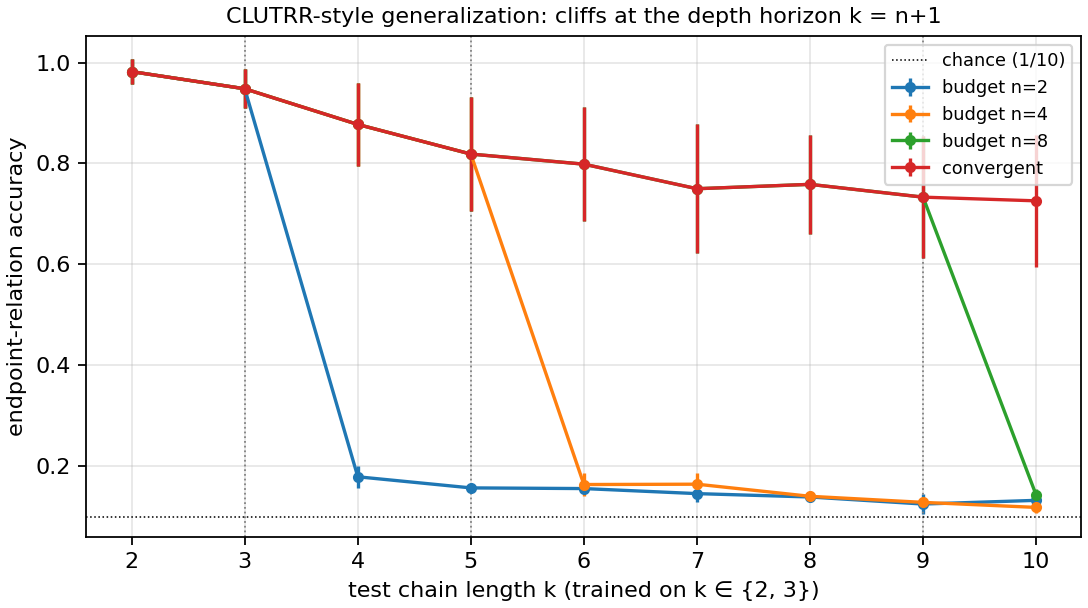
\includegraphics[width=.65\linewidth]{F11_clutrr.png}
\caption{E8: train on $k \le 3$, test long --- generalization cliffs at exactly the depth horizon,
with identical learned parameters across budgets.}
\label{fig:clutrr}
\end{figure}

%=====================================================================
\section{The hypothesis ledger}\label{sec:ledger}

The registered-prediction discipline, with outcomes. ``Toy'' marks results verified on the frozen
first implementation and not yet re-run on the rebuilt core.

\begin{center}\small
\begin{tabular}{llll}
\toprule
\# & prediction (sign / law) & source & outcome\\
\midrule
H1 & proof-sum over-counts; $\uparrow$ overlap; Bonferroni bound & Prop.~\ref{prop:addmult} &
\statusgood{confirmed} (E1, battery)\\
H2 & top-$k$ under-counts by dropped mass; $0$ iff $P \le k$ & Prop.~\ref{prop:topk} &
\statusgood{confirmed} (E1, controls)\\
H3 & crossover: ranking flips with overlap & underdetermined & \statusgood{confirmed}
($c \in (1,2)$)\\
H4 & min-max error sign structure-dependent & underdetermined & \statusgood{confirmed} (toy)\\
H5 & truncation: $0$ value, $0$ gradient below horizon $n{+}1$ & Prop.~\ref{prop:trunc} &
\statusgood{confirmed} (E2, E7, E8)\\
H6 & LSE bias $= \tau\ln P$; bias/liveness dilemma & Prop.~\ref{prop:lse} &
\statusgood{confirmed} (E3)\\
H7 & sum-product on cycles leaves $[0,1]$ ($\to 3.79$) & Thm.~\ref{thm:unbounded} gap &
\statusgood{confirmed} (E2)\\
H8 & inference error propagates to calibration/transfer & open & \statusgood{confirmed}
(E6 both, E5)\\
H9 & MNIST-sum-shaped tasks blind to double-counting & Prop.~\ref{prop:addmult} &
\statusgood{confirmed} (all controls)\\
H10 & non-stratified negation: outside claimed semantics & scope & toy demo only\\
H-A & top-1's setting dependence due to supervision richness & registered &
\textbf{refuted} (toy): parameterization\\
H-N/P1 & top-1 advantage decays monotonically with noise & registered & \textbf{refuted} (E5b):
knife-edge collapse\\
H-N/P2 & ranking reverses by $\eta = 0.5$ & registered & \statusgood{confirmed} (E5b)\\
F-1 & (discovered) addmultprob: tuple-fixpoint truncation & --- & \statusgood{measured + probed}\\
F-2 & (discovered) diffaddmultprob: straight-through clamp & --- & \statusgood{measured + confirmed}\\
\bottomrule
\end{tabular}
\end{center}

%=====================================================================
\section{Relation to prior work}\label{sec:related}

\paragraph{Semiring provenance and AMC.} Green et al.\ (2007) introduced provenance semirings;
Kimmig, Van den Broeck \& De Raedt (2017) separate circuit structure from semiring evaluation and
explain when sum-product is correct; Bourgaux et al.\ (2022) compare semantics for semiring
provenance under Datalog recursion; Khamis et al.\ (2024) analyze convergence of Datalog over
(pre-)semirings. Our algebra is inherited from this lineage (Remark~\ref{rem:attribution}); none
of these works measure deployed systems against claimed semantics.

\paragraph{Substrates.} Scallop (Li, Huang \& Naik, PLDI 2023) makes the provenance a runtime
choice; Lobster (2026) accelerates the same on GPUs; DeepLog (Derkinderen, Manhaeve et al., 2025;
software framework 2026) compiles NeSy specifications to algebraic circuits as a universal
backend, with DeepProbLog (Manhaeve et al., 2018) as a system layer. Substrates \emph{execute}
semantics; they make the question ``what does this flag actually compute, and what does it do to
learning?'' more urgent, not less. We measure all three (\S\ref{sec:conformance}); the analogy is
conformance test suites vs compilers --- different artifacts, both infrastructure.

\paragraph{Analyses of NeSy operators and losses.} Van Krieken et al.\ (AIJ 2022) analyze
differentiable fuzzy operators; van Krieken et al.\ (ICML 2024) and Faronius \& Dos Martires
(2025) debate the independence assumption at the \emph{loss} level, theory-first. Our instrument
is model-level and oracle-grounded; the E6/E5 transfer experiments supply controlled-structure
evidence that the loss-level debate lacks.

\paragraph{Benchmarks and assurance.} rsbench (NeurIPS D\&B 2024) targets perception-side
reasoning shortcuts --- orthogonal to our reasoning-side axis. The PNNL assurance study of Scallop
(2025) swept $k$ but measured calibration against accuracy rather than against the exact
marginal; our autopsy explains its null result: on sum-structured tasks the dominant failure mode
is invisible in principle. CLUTRR (Sinha et al., 2019) and GraphLog instantiate the depth axis in
natural-language form; E8 is our controlled stand-in, real-text CLUTRR remains future external
validity.

%=====================================================================
\section{Limitations, gaps, and threats to validity}\label{sec:limitations}

\begin{enumerate}[leftmargin=2em]
\item \textbf{Scope.} Rule/proof-based NeSy with monotone cores. Logic-as-loss systems (semantic
loss), non-rule NeSy, and non-monotone semantics (ASP, well-founded) are out of scope; stratified
negation exists only as a toy demo (H10) and has \emph{not} been ported to the rebuilt engine.
\item \textbf{Recursion coverage of the reference SUTs.} Finding~\ref{find:scallop} shows deployed
add-mult under recursion needs a truncated-at-tuple-fixpoint reference variant; it is specified
but not yet implemented, so recursive overlap sweeps against Scallop would currently use a wrong
reference model.
\item \textbf{Calibration needs synthetic perception.} Exact calibration requires closed-form
posteriors; on real images we measure perception MAE and transfer only (E5), and the E5b noise
injection is our device for restoring exactness on real data. This is a measurement-design
constraint, not an accident.
\item \textbf{Statistical depth.} Learning runs use 3 seeds (5 for the fact table); the headline
separations are many standard deviations wide, but the protocol's 5-seed standard is not yet met
everywhere. MNIST-sum control variances are large ($\pm0.14$ transfer) because two of three seeds
sit in a degenerate optimum --- worth more seeds before quoting.
\item \textbf{Toy-only results.} The H-A supervision-richness ablation and the H4 sign-dependence
numbers are verified on the frozen toy but not yet re-run on the rebuilt core (everything else in
this report is rebuilt-core output).
\item \textbf{Adapters not yet exercised.} Scallop's torch-tagged \texttt{diff*} provenances
(beyond finite differences); DeepLog's fuzzy/G\"odel structures; a standalone (pre-DeepLog)
DeepProbLog audit; Lobster.
\item \textbf{E8 is CLUTRR-style, not CLUTRR.} Lineal fragment, own generator, no text layer ---
stated wherever it appears; real-text CLUTRR is future work.
\item \textbf{Internal vs external validity.} The toy$\leftrightarrow$rebuild decimal-exact
replication is \emph{internal} (shared seeds and math). External anchors: ProbLog agreement
($10^{-16}$), Scallop agreement ($10^{-16}$), DeepLog agreement ($10^{-7}$), each on independent
codebases. Our adapters could still misuse an upstream API; for the Scallop finding we therefore located the mechanism in its evaluation policy and built a minimal witness, rather than resting on
black-box disagreement.
\item \textbf{The brute-force oracle caps at 22 facts.} Larger instances use ProbLog; learning
structures cap at 16 facts ($2^m$ world enumeration). Scaling the oracle (compilation-based) is open.
\item \textbf{Generality of generators.} G1--G3 are designed families, chosen to isolate axes;
random-program sweeps (random DAGs from the protocol) are not yet productionized.
\end{enumerate}

%=====================================================================
\section{Anticipated questions}\label{sec:faq}

\begin{question}[``Isn't this just semiring PLP / the KR paper again?'']
The algebra is inherited and explicitly attributed (Remark~\ref{rem:attribution}); nothing here
re-proves it. What did not exist before: the fidelity definitions (D1--D6), the error laws as
\emph{registered} signed predictions, the structure-controlled generators with exact oracles and
analytic gradients, the conformance measurements of deployed systems (a finding), and the
learning-consequence results. None of these are derivable from the theorems --- two of our own
registered predictions were refuted by measurement.
\end{question}

\begin{question}[``Is this DeepLog? Why is your instrument not redundant given their framework?'']
DeepLog executes a chosen semantics by compilation; it does not measure whether a deployed system
matches its claim, and it cannot be the neutral referee for its own stack. We measured DeepLog
itself: its core passes conformance (including gradients). A substrate and a test suite are different artifacts;
the existence of good compilers does not make conformance suites redundant.
\end{question}

\begin{question}[``The error laws are trivial.'']
Individually, yes --- deliberately (we say so in \S\ref{sec:laws}). The non-trivial content is
(i) what they underdetermine (crossover location, min-max sign, every learning-time interaction),
(ii) their conversion into an instrument with exact oracles, and (iii) the measured consequences:
accuracy-invisible miscalibration, gradient starvation, benchmark blindness, knife-edge regime
dependence.
\end{question}

\begin{question}[``Could your finding be a bug in your adapter rather than in the system?'']
We (a) reproduced at machine precision the cells where Scallop agrees with its claim (so the
adapter is demonstrably faithful elsewhere), (b) designed a minimal witness (the diamond probe
isolating tuple-set truncation), and (c) located the mechanism in the upstream evaluation
policy (semi-naive iteration to the tuple-set fixpoint). The finding is a claim about a pinned
version, guarded by canary tests.
\end{question}

\begin{question}[``Why are the synthetic perception experiments not a weakness?'']
Because calibration against \emph{exact} posteriors is the quantity of interest and only a known
generative model provides it. The MNIST experiments (E5) show the findings survive real images;
the noise ablation (E5b) shows how to recover exact ground truth on real data by owning the
stochasticity. The instrument's claim is about reasoning-layer fidelity, which is exactly what
this design isolates.
\end{question}

\begin{question}[``Accuracy ties: maybe your tasks are just too easy/hard?'']
The ties occur at accuracies far from both chance and ceiling ($0.73$--$0.75$ synthetic, $0.93$--%
$0.95$ MNIST), and the same trained pipelines are separated decisively by calibration and
transfer. The mechanism is structural --- monotone distortions preserve rankings --- not a
ceiling artifact.
\end{question}

\begin{question}[``Why should anyone adopt this rather than just being careful?'']
F-\ref{find:scallop} occurred in a careful, well-engineered system by a strong group; H-A and H-N/P1 were wrong expectations held by people who had just built the
instrument. ``Being careful'' does not produce signed, oracle-grounded, regression-pinned
measurements; a 30-line adapter does (\texttt{docs/ADAPTERS.md}).
\end{question}

\begin{question}[``What would falsify the headline claim?'']
A structured family on which a non-exact aggregation matches exact calibration/transfer while its
inference-time $\lvert\eps\rvert$ is large (breaking H8's propagation), or a deployed system whose
measured semantics contradicts our reference model on the acyclic battery (breaking the
conformance transfer). Both are exactly what the instrument is built to detect --- and publishing
them would be a result, as E5b shows.
\end{question}

%=====================================================================
\section{Roadmap}\label{sec:roadmap}

(i) Close the gaps that block claims: truncated-fixpoint reference variant for recursive add-mult;
port H-A and negation to the rebuilt core; 5 seeds everywhere; more seeds on the MNIST control.
(ii) Externalize: arXiv the theory
companion once KR decisions allow; venue per the standing plan (AAAI-27 cycle next).
(iii) Extend: Scallop \texttt{diff*} gradients via torch tags; DeepLog fuzzy structures; Lobster;
real-text CLUTRR; random-DAG sweeps; compilation-based oracle beyond 22 facts.

\appendix
%=====================================================================
\section{Notation}\label{app:notation}

\begin{center}\small
\begin{tabular}{ll}
\toprule
$\Sigma$, $\HB(\Sigma)$ & signature; Herbrand base (Def.~2.1)\\
$\mathcal P$; $q$ & ground program; query atom (Def.~\ref{def:program})\\
$(V,\oplus,\otimes,0,1)$ & commutative semiring; $\otimes$ body composition, $\oplus$
aggregation (Def.~\ref{def:semiring})\\
$f_\theta$ & base interpretation: EDB values from perception; $0$ on IDB
(Def.~\ref{def:base})\\
$T_{\mathcal P}$, $F^{f_\theta}_{\mathcal P}$, $I^{(n)}$ & consequence operator; fact-augmented
operator; $n$-step iterate (Def.~\ref{def:tp})\\
$\pi$, $\mathrm{depth}$, $\val$, $\mathrm{supp}$ & proof tree, its depth, value, support
(Def.~\ref{def:proofs})\\
$\Infer^{(n)}(q)$ & depth-bounded proof aggregation (Def.~\ref{def:proofs})\\
$I^\star$, $\lfp$ & least-fixed-point semantics (Thm.~\ref{thm:unbounded})\\
$P^*(q)$, $\pi(w)$ & distribution-semantics value (WMC); world probability
(Def.~\ref{def:wmc})\\
$\sigma_j$, $s_j$, $E_j$ & proof support; score $\prod_{f\in\sigma_j}p_f$; event
$\bigwedge_{f \in \sigma_j} f$\\
$P, L, c, p$ & G1 parameters: \#proofs, length, shared trunk, probability\\
$\hat\sut(q)$, $I^*(q)$, $\eps_\sut(q)$ & SUT value; oracle value under the claim; semantic
error (Def.~\ref{def:error})\\
$\phi_a(\sut)$, $h_\delta$, live & fidelity profile, depth horizon, gradient liveness
(Defs.~\ref{def:profile}--\ref{def:liveness})\\
$\mathrm{LSE}_\tau$ & $\tau\log\sum_j e^{s_j/\tau}$ (Def.~\ref{def:suts})\\
$\eta$ & latent label-noise rate (E5b)\\
$k$; $n$ & chain length (E8) / top-$k$ size; unrolling budget\\
\bottomrule
\end{tabular}
\end{center}

\section{Reproduction}\label{app:repro}

\texttt{python3 -m venv .venv \&\& .venv/bin/pip install -e ".[dev,oracles,reporting]"}, then
\texttt{make all} (tests $\to$ E1--E4 $\to$ E6/E7 $\to$ E5/E5b $\to$ E8 $\to$ scorecard + report).
Every experiment is a committed YAML config whose sha256 is embedded in its JSON output; figures
regenerate from the JSONs; \texttt{out/RESULTS.md} is auto-generated. Version pins for the
deployed systems are recorded in the conformance logs (\texttt{out/conformance\_scallop.md},
\texttt{out/conformance\_deeplog.md}, \texttt{out/conformance\_problog\_kbest.md}, \texttt{out/conformance\_deepproblog.md}, \texttt{out/conformance\_ltn.md}). The frozen first
implementation lives under \texttt{legacy/} with the golden parity fixtures under
\texttt{tests/fixtures/}.

\begin{thebibliography}{24}\small
\bibitem{vEK} M.~van Emden, R.~Kowalski. The semantics of predicate logic as a programming
language. \emph{J.\ ACM} 23(4), 1976.
\bibitem{Lloyd} J.~Lloyd. \emph{Foundations of Logic Programming}, 2nd ed. Springer, 1987.
\bibitem{Green} T.~Green, G.~Karvounarakis, V.~Tannen. Provenance semirings. \emph{PODS}, 2007.
\bibitem{Kimmig} A.~Kimmig, G.~Van den Broeck, L.~De Raedt. Algebraic model counting.
\emph{J.\ Applied Logic} 22, 2017.
\bibitem{DM} A.~Darwiche, P.~Marquis. A knowledge compilation map. \emph{JAIR} 17, 2002.
\bibitem{Bourgaux} C.~Bourgaux, P.~Bourhis, L.~Peterfreund, M.~Thomazo. Revisiting semiring
provenance for Datalog. \emph{KR}, 2022.
\bibitem{Khamis} M.~Abo Khamis, H.~Ngo, R.~Pichler, D.~Suciu, Y.~Wang. Convergence of Datalog
over (pre-)semirings. \emph{J.\ ACM} 71(2), 2024.
\bibitem{Sato} T.~Sato. A statistical learning method for logic programs with distribution
semantics. \emph{ICLP}, 1995.
\bibitem{ProbLog} L.~De Raedt, A.~Kimmig, H.~Toivonen. ProbLog: a probabilistic Prolog and its
application in link discovery. \emph{IJCAI}, 2007.
\bibitem{DeepProbLog} R.~Manhaeve, S.~Duman\v{c}i\'c, A.~Kimmig, T.~Demeester, L.~De Raedt.
DeepProbLog: neural probabilistic logic programming. \emph{NeurIPS}, 2018.
\bibitem{Scallop} Z.~Li, J.~Huang, M.~Naik. Scallop: a language for neurosymbolic programming.
\emph{PLDI}, 2023.
\bibitem{Lobster} Lobster: a GPU-accelerated framework for neurosymbolic programming.
\emph{ASPLOS}, 2026. arXiv:2503.21937.
\bibitem{DeepLogA} V.~Derkinderen, R.~Manhaeve, et al. The DeepLog neurosymbolic machine.
arXiv:2508.13697, 2025.
\bibitem{DeepLogB} DeepLog: a software framework for modular neurosymbolic AI. arXiv:2605.10279,
2026 (IJCAI demo).
\bibitem{vK22} E.~van Krieken, E.~Acar, F.~van Harmelen. Analyzing differentiable fuzzy logic
operators. \emph{AIJ} 302, 2022.
\bibitem{vK24} E.~van Krieken, P.~Minervini, E.~Ponti, A.~Vergari. On the independence assumption
in neurosymbolic learning. \emph{ICML}, 2024.
\bibitem{Faronius} H.~Faronius, P.~Z.~Dos Martires. Independence is not an issue in
neurosymbolic AI. 2025.
\bibitem{rsbench} S.~Bortolotti et al. A benchmark suite for systematically evaluating reasoning
shortcuts. \emph{NeurIPS D\&B}, 2024.
\bibitem{PNNL} Assurance of reasoning-enabled AI systems: an analysis of Scallop.
arXiv:2502.08932, 2025.
\bibitem{CLUTRR} K.~Sinha, S.~Sodhani, J.~Dong, J.~Pineau, W.~Hamilton. CLUTRR: a diagnostic
benchmark for inductive reasoning from text. \emph{EMNLP}, 2019.
\bibitem{NTP} T.~Rockt\"aschel, S.~Riedel. End-to-end differentiable proving. \emph{NeurIPS},
2017.
\bibitem{TensorLog} W.~Cohen. TensorLog: a differentiable deductive database. 2016.
\bibitem{SL} J.~Xu, Z.~Zhang, T.~Friedman, Y.~Liang, G.~Van den Broeck. A semantic loss function
for deep learning with symbolic knowledge. \emph{ICML}, 2018.
\bibitem{QuickCheck} K.~Claessen, J.~Hughes. QuickCheck: a lightweight tool for random testing of
Haskell programs. \emph{ICFP}, 2000.
\end{thebibliography}

\end{document}
